\subsection*{RQ3: Can logrn churn metrics help in explaining the resolution time of bugs?} 

\subsubsection*{Motivation}
%Prior research has shown that resolution time is correlated to the number of developers and the number of comments in an issue report~\cite{RTpredictions}. However, prior research does not look at the type of changes made by developers. 

In RQ2, we find that bug fixes with log changes take shorter time to get resolved than bug fixes without log changes. However, there may be confounding effects between metrics, i.e., resolution time, total churn, \# of developers and \# of discussions, such that it is difficult to draw unbiased conclusion on the relationship between resolution time and log changes. To further explore this relationship between resolution time and log changes in bug fixes, we build prediction models using metrics from prior research and log churn metrics. %We want to understand the effect of log changes during bug fixes and also identify which types of log changes can be beneficial during bug fixes. 

\subsubsection*{Approach}

To better understand the relationship between log changes and the resolution time for fixing bugs, we build a non-linear regression model. Prior research has shown that linear modelling can help in predicting the resolution time of bugs~\cite{anbalagan2009predicting}. However, the relationship between resolution time of bug fixes and log changes may be non-monotonic. By building a non-linear regression model we can more appropriately approximate the relationship between resolution time and log churn metrics, during bug fixes.

A non-linear regression model fits the curve of the form $y = \alpha + \beta_{1}x_{1} + \beta_{2}x_{x} + .. + \beta_{n}x_{n} $ to the data, where $y$ is the dependent variable (i.e., resolution time of bugs) and every $x_{i}$ is an explanatory metrics. The explanatory metrics include the log churn metrics (as shown in RQ1). Since prior research finds that the number of developers and the number of comments in an issue report are correlated to the resolution time of the issue report, we include the number of developers and the number of comments as explanatory metrics. We find that bugs with more complex fixes may take longer time to resolve (see RQ2). Therefore, we also include code churn as an explanatory metric. We use the \textsl{rms} package~\cite{rmsPackage} from R, to build non-linear regression models. The overview of our modeling process is shown in Figure~\ref{fig:MethodologyOLS} and is explained below. 




% In our model, \textsl{resolution time} is the dependent variable $y$ and the log churn metrics are the explanatory variables.


\noindent \textbf{(1) Calculating the degrees of freedom}

During predictive modeling, a major concern is over-fitting. An over-fit model is biased towards the dataset from which it is built and will not well fit other datasets. In non-linear regression models, over-fitting may creep in when an explanatory metric is assigned more degrees of freedom than the data can support. Hence, it is necessary to calculate a budget of degrees of freedom that a dataset can support before fitting a model. We budget $\frac{x}{15}$ degrees of freedom for our model as suggested by prior research~\cite{DegreesofFreedom}, where \textsl{x} is the number of rows (i.e, \# bugs) in each project. 


\noindent \textbf{(2) Correlation and redundancy analysis}

Correlation analysis is necessary to remove the highly correlated metrics from our dataset. We use Spearman rank correlation to assess the correlation between the metrics in our dataset. We use Spearman rank instead of Pearson correlation because Spearman rank correlation is resilient to data that is not normally distributed. We use the function \textsl{varclus} in R to perform the correlation analysis. From the hierarchical overview of explanatory metrics constructed by the \emph{varclus} function, we exclude one metric from the sub-hierarchies which have correlation $|\rho| > 0.7 $.
% \ian{what's your cutoff and how do you decide which metrics to remove, check what shane wrote.}

Correlation analysis does not indicate redundant metrics, i.e, metrics that can be explained by other explanatory metrics. The redundant metrics can interfere with the one another and the relation between the explanatory and dependent metrics is distorted. We perform redundancy analysis to remove such metrics. We use the \textsl{redun} function that is provided in the \textsl{rms} package to perform the redundancy analysis.

\begin{figure}
	\centering
	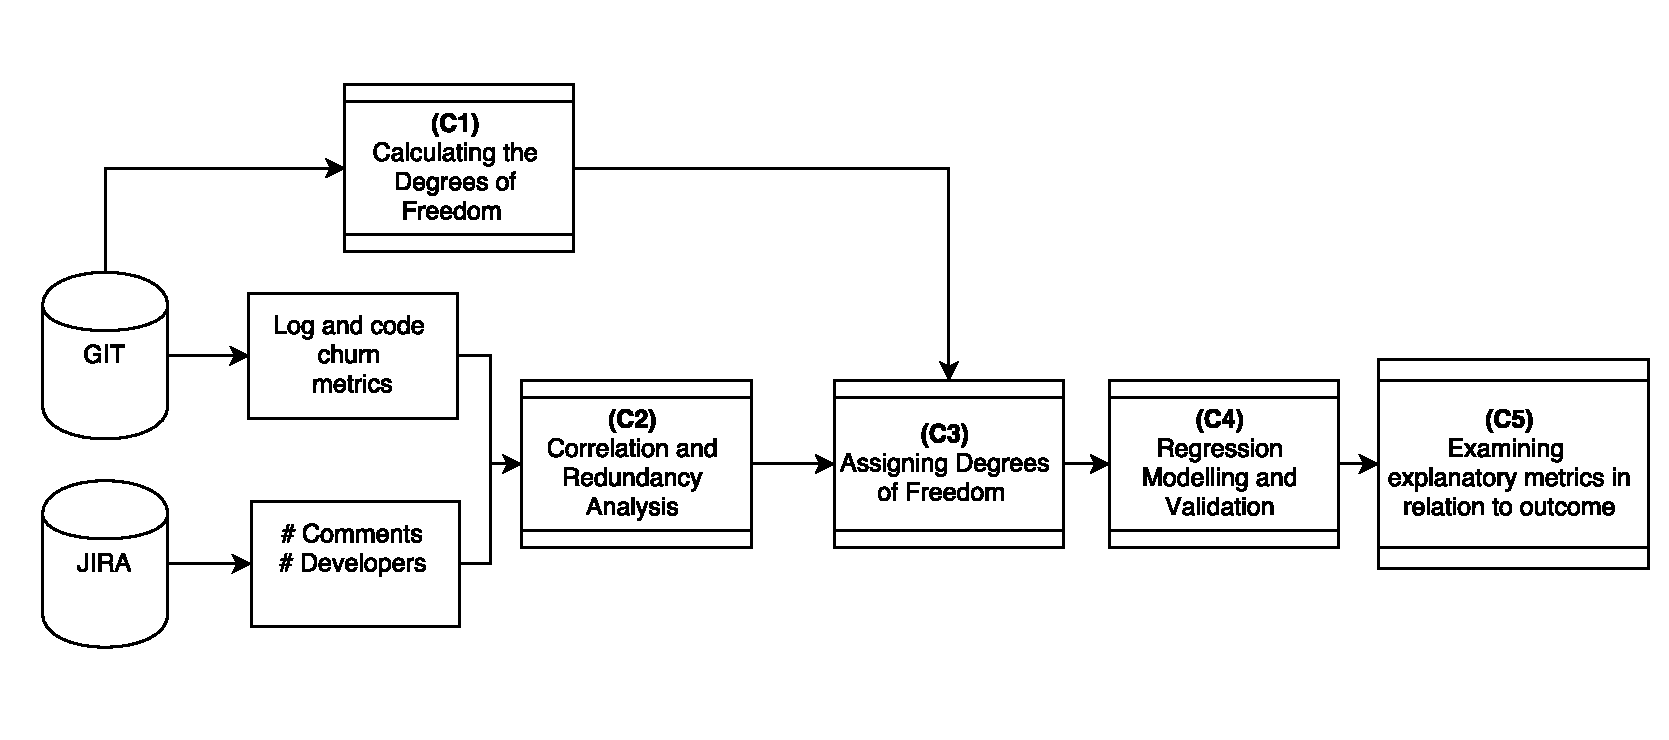
\includegraphics[width=9.8cm]{MethodologyOLS}
	\caption{Overview of our non-linear OLS model construction(C) for the resolution time of bugs}
	\label{fig:MethodologyOLS}
\end{figure}



\noindent \textbf{(3)Assigning degrees of freedom}


After removing the correlated and redundant metrics from our datasets, we spend the budgeted degrees of freedom efficiently. We identify the metrics which can use the benefit from the additional degrees of freedom (knots) in our models. To identify these metrics we use the Spearman multiple $\rho^{2}$ between the explanatory and dependent metrics. A strong relation between explanatory metrics $x_{i}$ and the dependent metric $y$ indicates that, $x_{i}$ will benefit from the additional knots and improve the model. We use the function \textsl{spearman} in the \textsl{rms} package to calculate the Spearman multiple $\rho^{2}$ values for our metrics (metrics with larger $\rho^{2}$ values are allocated more degrees of freedom than metrics with smaller $\rho^{2}$ values).

\noindent \textbf{(4)Regression modeling and validation}

After budgeting degrees of freedom to our metrics we build a non-linear regression model using the function OLS (Ordinary Least Squares) that is provided by the \textsl{rms} package. We use the \textsl{restricted cubic splines} to assign the knots to the explanatory metrics in our model. 
As we are trying to identify the relationship between log churn metrics and the resolution time of bug fixes, we are primarily concerned if the log churn metrics are significant in our models. Therefore, we use chunk test (a.k.a Wald test) to determine the statistically significant metrics to included in our final model. We choose chunk test as some of our explanatory variables are allocated several degrees of freedom and have to be tested jointly, similar to previous research~\cite{ShaneOLS}. At each step in the Wald test, we measure the significance of each metric according to its p-value. We consider only those metrics that have p-values lower than 0.05 in the final model. We use \textsl{wald.test} function provided by the R package \emph{aod}~\cite{waldtest} to perform the chunk test.  


\noindent \textbf{(5) Examining explanatory metrics in relation to outcome}

After identifying the significant metrics in our datasets we find the relation between each explanatory metric and the resolution time of bugs. In our regression models, each explanatory metric can be explained by several knots assigned to that metric. To account for the impact of all knots associated with an explanatory metric, we plot the changes to resolution time against each metric, while holding the other metrics at their median value using the \emph{Predict} function in the \emph{rms} package~\cite{rmsPackage}. The plot follows the relationship as it changes directions at the spline (knot) locations (C-3). 

We would like to point out that although non-linear regression models can be used to build accurate models for the resolution time of bugs, our purpose of using the non-linear regression models in this paper is not for predicting the resolution time of bugs. Our purpose is to study the explanatory power of log churn metrics and explore their empirical relationship to the resolution time of bugs.%We controlled the metrics by total code churn. We used \textsl{Wilcoxon} test to measure the statistical significance of each metric in bugs fixed with log changes with bugs fixed without log changes. \textsl{Cohens.D} is used to measure the size of the difference of each metric. 



\subsection*{Results}

\begin{figure}[t]
	\centering 
	\begin{minipage}[b]{1\columnwidth}
			\centering 
			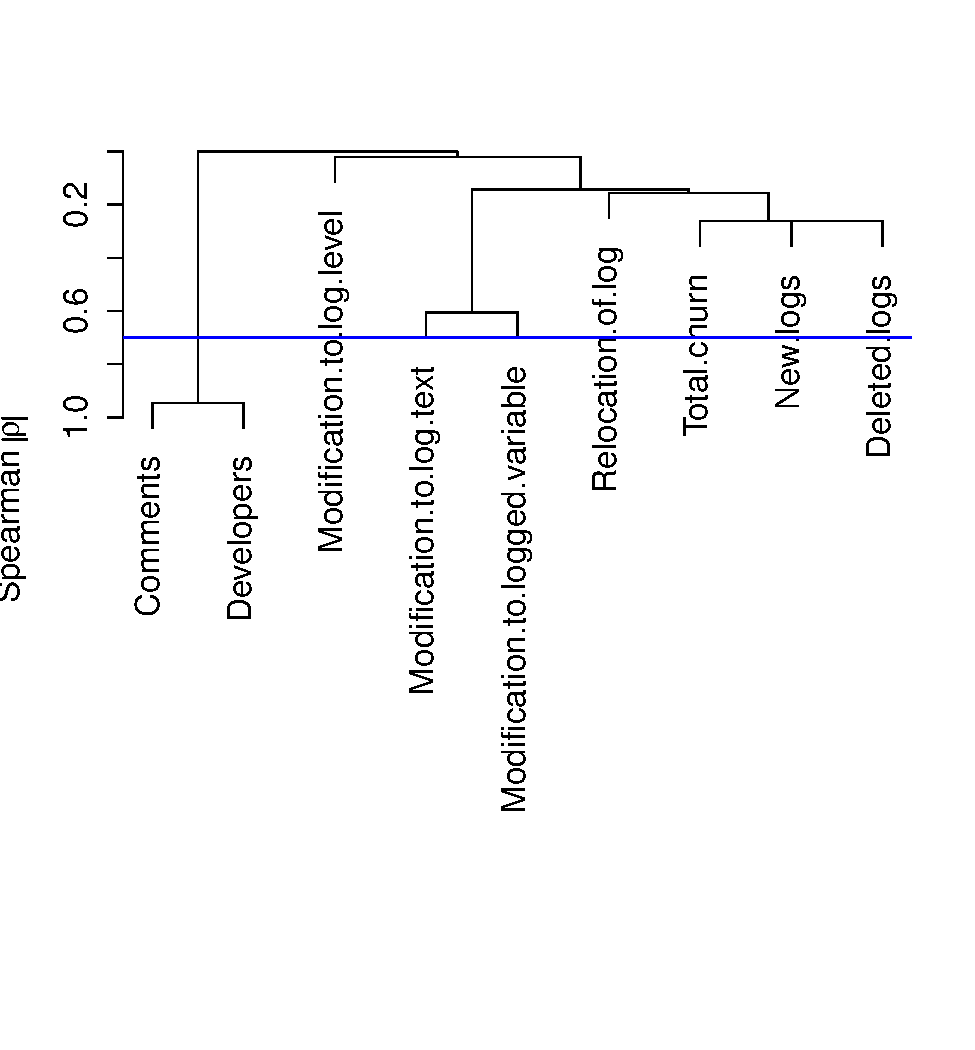
\includegraphics[width=.8\columnwidth]{QpidSpearman}	
		%		\subcaption{Correlation between metrics in Qpid}

	\end{minipage}
	
	\vspace*{-1.5cm}	\caption{Correlation between metrics in Qpid. Blue line indicates cut of set to 0.7\label{fig:Correlation}}
\end{figure}

In this subsection, we describe the outcome of the model construction and analysis outlined in our approach and Figure~\ref{fig:MethodologyOLS}

\textbf{(1) Calculating degrees of freedom}. Our data can support 123 ($\dfrac{1,925}{15}$ in Hadoop), 63($\dfrac{953}{15}$ in Qpid) and 183($\dfrac{2,755}{15} $ in HBase) degrees of freedom for the studied projects. As we have large degrees of freedom in each project, we can be liberal in the allocating splines (knots) to the explanatory variables during model construction. 


\textbf{{(2) Correlation and redundancy analysis}}. Figure~\ref{fig:Correlation} shows the hierarchically clustered Spearman $\rho$ values of the three systems. The blue line indicates our cut-off value ($|\rho|$ = 0.7 ). Our analysis reveals that \# \textsl{Comments} and \# \textsl{developers} are highly correlated in \emph{Qpid} and \emph{HBase}. We chose to remove \#\textsl{developers} from our model since \#\textsl{comments} is a simpler metric than \#\textsl{developers}. We find that there are no redundant metrics in our metrics in all the studied projects.


\textbf{(3) Assigning degrees of freedom}. Figure~\ref{fig:Spearman} shows the Spearman multiple $\rho^{2}$ of the resolution time against each explanatory metric. Metrics that have higher Spearman multiple $\rho^{2}$ have higher chance of benefiting from the additional degrees of freedom to better explain resolution time. Based on Figure~\ref{fig:Spearman}, we split the explanatory metrics into three groups. The first group consists of \#\textsl{comments}, the second group consists of \#\textsl{modifications to log level}, \#\textsl{ modifications to log variable}, \#\textsl{relocation of log} and \#\textsl{new logs}. The last group consists of the remaining metrics. We allocate five degrees of freedom i.e, knots, to the metrics in the first group, three to metrics in second group and no knots to metrics in last group similar to prior research~\cite{ShaneOLS}.


\begin{figure}[t]
	\begin{minipage}[b]{1\columnwidth}
			\centering 
		\hspace*{-2cm}	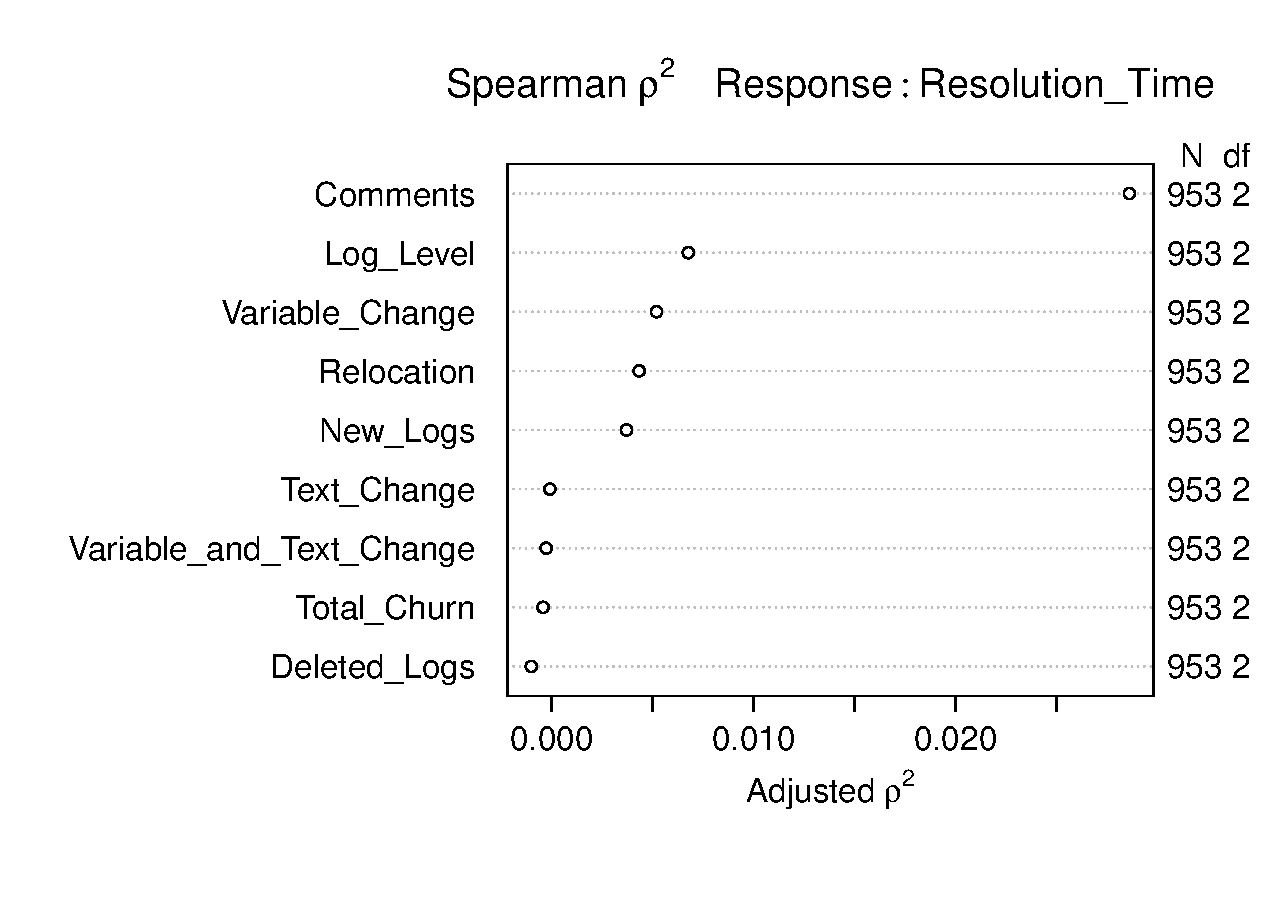
\includegraphics[width=0.7\textwidth]{QpidDF}	
		
	\end{minipage}
	\captionsetup{labelsep = colon}
	\hspace*{1.7cm}\caption{Spearman multiple $\rho^{2}$ of each explanatory metric against Resolution Time of bug fixes with log changes. Larger values indicate more potential for non-linear relationship \label{fig:Spearman}}
\end{figure}




\textbf{(4) Regression modeling and validation.} After allocating the knots to the explanatory metrics, we build the non-linear regression model and use the \textsl{validate} function in the \textsl{rms} package to find the significant metrics in our studied projects. We find that log churn metrics are significant in Qpid and HBase systems for predicting resolution time of bug fixes. 

\begin{figure*}[t]
	\begin{minipage}{.5\columnwidth}
		\centering
		
		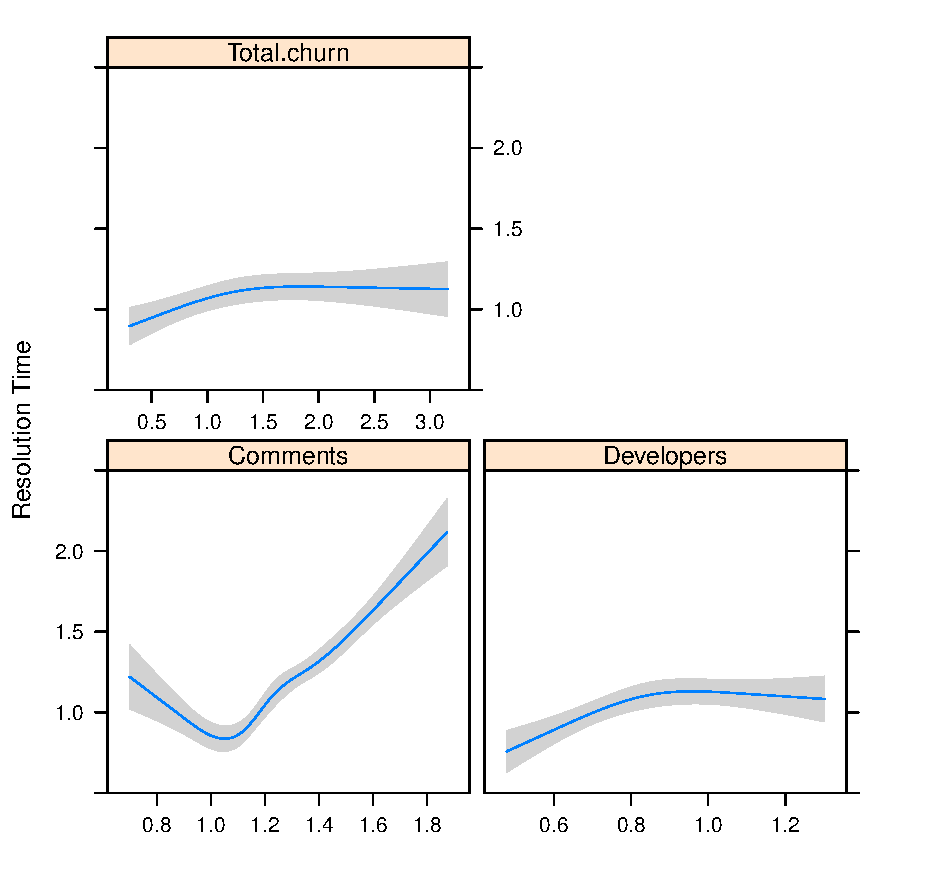
\includegraphics[width=.95\textwidth]{HadoopDirectionPlot}	
		\subcaption{Hadoop}
	\end{minipage}
		\begin{minipage}{.5\columnwidth}
			\centering
			
			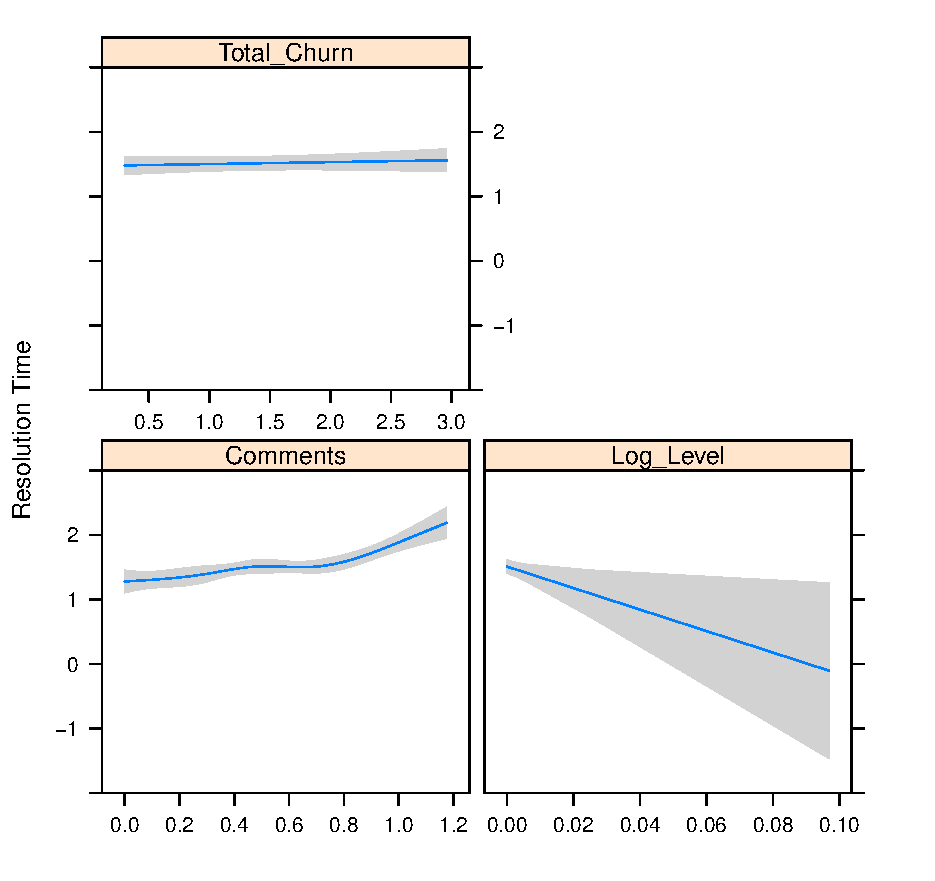
\includegraphics[width=.95\textwidth]{QpidDirectionPlot}	
			\subcaption{Qpid}
		\end{minipage}
			
	\begin{minipage}{0.5\columnwidth}
		\hspace*{1.9cm}	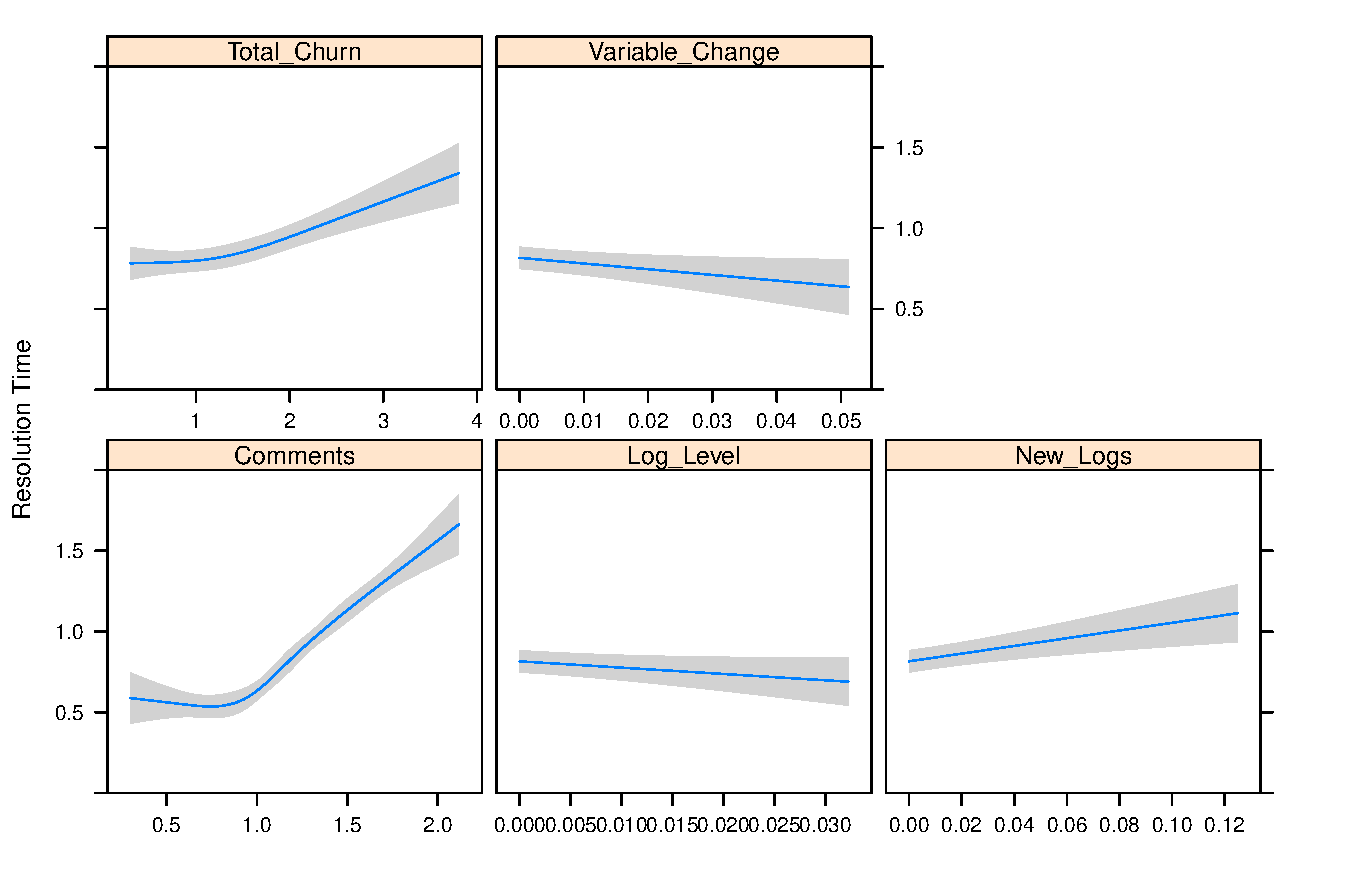
\includegraphics[width=1.45\textwidth]{HbaseDirectionPlot}
  \captionsetup[subfigure]{oneside,margin={3.5cm,-2.5cm}}

	\subcaption{HBase}
	\end{minipage}
	\hspace*{1.cm}\caption{Relation between the explanatory metrics and resolution time of bug fixing commits with log changes. Increasing graph shows increase in explanatory metrics increases the resolution time and decrease reduces the resolution time \label{fig:HbaseDirectionPlot}}
\end{figure*}

\textbf{(5) Examining explanatory metrics in relation to outcome}. Figure~\ref{fig:HbaseDirectionPlot} shows the direction of impact of log churn metrics on the resolution of bug fixes with log changes in \emph{HBase}. We find that log modifications have a negative impact on the resolution time of bug fixes. Shown in Figure~\ref{fig:HbaseDirectionPlot}, we find that in \emph{HBase} and \emph{Qpid}, modifications to logs, i.e, log level changes and variable changes are significant in the models and have negative correlations with the resolution time of bugs. 

\textbf{Modifications to log level have a negative relationship with bug resolution time.} 
We find that modifications to log level have statistically significant explanation power to bug resolution time for \emph{Qpid} and \emph{HBase}. Even though developers often do not modify log levels during bug fixes (see RQ1), our results show that changes to log levels may help in faster resolution of bugs. Although prior research finds that developers are confused when estimating the cost and benefit of each verbosity level in a log~\cite{Characterizinglogs}, a properly chosen log level may help developers diagnose filed bugs. On the other hand, a improper log level may result in too little or too much log, which are considered undesirable for diagnosing bugs~\cite{zhao2014lprof,Fu1}. An example where developers overestimate the log verbosity level is in the issue HBASE-8359\footnote{https://issues.apache.org/jira/browse/HBASE-8359}, where the log is set to \emph{info} and causes confusion among system administrators. We find that developers change the log verbosity level from \emph{info} to \emph{trace}, to reduce bulk logs being generated. On the other hand in HBASE-3401\footnote{https://issues.apache.org/jira/browse/HBASE-3401}, we see that developers underestimate the verbosity level and the log is set to default \emph{debug} and has to be updated to \emph{warn} to give more priority to the logged event. 

\textbf{Modifications to logged variables have a negative relationship with bug resolution time.} 
We find that variable changes have a statistically significant explanation power in the model for \emph{HBase} with negative relationship on the resolution time of bugs. This may be because changing information in the logs may benefit developers during bug fixes. The other reason may be that developers add new functions or keywords and leverage the new information in the logs to ensure the functionality of the new code and assure the bug is fixed~\cite{Fu1}. This enables developers to resolve the issue faster. In RQ1, we find that variable changes; especially addition and modification of logged variables is higher in bug fixes than non-bug fixes. These modifications to the logged variables highlight that developers have recognized the importance of information that is printed from logs and act on improving logs in order to assist in bug fixing.


%\begin{table}[t]
%	
%	\caption{Effect of log churn metrics on resolution time of bugs. Effect is measured by adding one standard deviation to its mean value, while the other metrics are kept at their mean values.}
%	\label{tba:SignificantFactor}
%	\begin{tabular}{|>{\centering}p{.08\textwidth}>{\centering}p{.21\textwidth}|>{\centering}p{.1\textwidth}>{\centering}p{.15\textwidth}|>{\centering}p{.1\textwidth}>{\centering}p{.15\textwidth}|}
%		\hline 
%		Delta Y  & Variable & Delta Y  & Variable & Delta Y  & Variable\tabularnewline
%		\hline 
%		\textbf{Qpid} &  & \textbf{Hadoop} &  & \textbf{HBase} & \tabularnewline
%		0.0996  & \# Comments & 0.2741  & \# Comments & 0.3562  & \# Comments\tabularnewline
%		-0.0691  & Log Level Changes & 0.0258 & Total Churn & 0.1157 & Total Churn\tabularnewline
%		&  & 0.0191  & Developers & 0.0517 & New Logs \tabularnewline
%		&  &  &  & -0.0281 & Log Level Changes\tabularnewline
%		&  &  &  & -0.0367 & Variable Changes\tabularnewline
%		\hline 
%	\end{tabular}
%	\par
%\end{table}
\textbf{New logs have a positive relationship with bug resolution time.} 
We find that new logs have a statistically significant explanation power in the model for \emph{HBase} with a positive relationship on the resolution time of bug fixes. We find that logs are often added during bug fixes in order to verify the quality of the bug fixing code. From our manual analysis results of RQ2, we find that such bugs are often complex to fix, with a large amounts of code churn and long resolution time. We compare the average code churn of bug fixes with new logs and bug fixes without new log additions. We find that the average code churn of bug fixes with new logs is almost twice that of average code churn of bug fixes without new log additions. For example, in HBASE-7305\footnote{https://issues.apache.org/jira/browse/HBASE-7305}, developers implement a read write lock for table operations to fix a race condition. This issue has total code churn over 2.5 K with over 70 new logs in the code. Because of the addition of new features this issues takes over two months to be resolved with 44 discussion posts on the issue. 


\hypobox{Log churn metrics can complement the number of comments, the number of developers and total code churn in modelling the resolution time of bugs. We find that modifications to logged variables and modifications to log level have a negative relationship with resolution time of bug fixes. On the other hand, the new logs have a positive relationship with resolution time of bugs.}

